\section{Ethereum Basics}

\subsection{Smart Contract}
Ethereum \cite{ethereumyellow} is a decentralised state machine. Where transactions in Bitcoin update balances of accounts, Ethereum transactions update the state of a tree structure. These state transitions allow for Turing completeness, meaning arbitrary code can be executed on the blockchain. This is used to make smart contracts, pieces of code living on the Ethereum network, that anyone can interact with. One of the most popular usecases is to make tokens that can be traded between users trustlessly. To facilitate interoperability with these tokens and other smart contracts, they usually adhere to a standard, known as ERC20. Ethereum Request for Comment (ERC) \cite{erc} is much like RFCs \cite{httprfc} that describe internet protocols like HTTP and TCP/UDP. 

\subsection{Transactions and gas}

When you want to transact on the Ethereum network, you sign a transaction with a certain gas price. The gas price is the price you are willing to pay per unit of computation your transaction requires. Every operation has a certain weight associated with it (ie. a multiplication cost X gas) and the gas price is the amount you are willing to pay per gas.
After the London upgrade, which introduced \cite{eip1559}, every block has a base fee. This means that if you are not willing to pay at least the base fee in gas price, your transaction cant be included in the block. The base fee fluctuates over time, so it might be enough to wait for the base fee to go down. If you pay more than the base fee in gas price for your transaction, the excess will be taken by the miner. The base fee always gets burned, meaning that every transaction removes some Ether from the supply. 

\subsection{Decentralised Exchanges and Arbitrage}
A Decentralised Exchange (DEX) is a smart contract that allows for users to trade an asset for another (usually ERC20 tokens). Historically, many different DEX designs have been used, but the most popular is the Automated Market Maker (AMM). Uniswap is an example of an AMM \cite{uniswap}. Uniswap holds token reserves of different ERC20's in what are called pools. If a users buys token A for token B, the next time a users wants to do the same, the price of A denominated in B has increased, meaning the second user gets less of token A than the first user did. Similarly, if a user sells token A for B, the price of A denominated in B decreases, and a second user that wants to buy token A, will now get more of it. If the same pair of tokens exists on multiple DEX's, there exist arbitrage opportunities. If the price of A denominated in B is lower on one exchange, users can make a profit by buying token A there, and selling it for a higher price on a different exchange. 

\subsection{Transaction Ordering}
When you want to transact on the Ethereum network, the traditional way of doing so is by submitting a transaction to the mempool. This transaction is then propagated through the P2P network of Ethereum nodes, to be considered for inclusion by miners. Traditionally the ordering of transactions in a block was sorted by the highest gas price. The journey of a transaction looks like this: 

\begin{figure}[H]
    \centering
    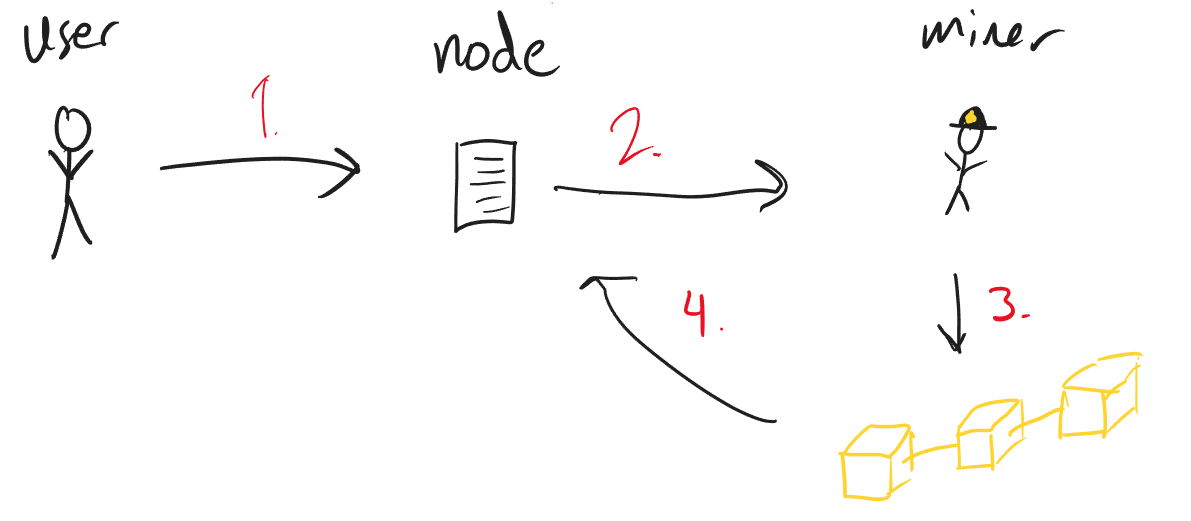
\includegraphics[width=\textwidth]{3_FIGURES/Theory/Transaction1.PNG}
    \caption{Transaction life cycle}
    \label{transaction1}
\end{figure}

\begin{enumerate}
    \item First a user signs a transaction (usually with a hardware or software wallet) and sends it through Remote Procedure Call (RPC) to an Ethereum node.
    \item The Ethereum node then propagates the transaction to other nodes in the network. Some of those nodes belong to miners/mining pools.
    \item The miners consider the transaction for inclusion in the next block. If the the gas price the user is willing to pay for the transaction is large enough, the transaction gets included in a block.
    \item The miner propagates the found block to the network, and the user can use RPC to see their transaction in the new block through the node they initially submitted the transaction to.
\end{enumerate}


\subsection{Priority Gas Auction}

Miners include transactions in blocks to make profit. If the users do not submit transactions that have a gas price greater than the base fee, there is no real incentive for the miners to include them. Miners have traditionally included the transaction with the highest gas fee in descending order of gas fees. This tradition lead to something dubbed Priority Gas Auctions (PGA's) in the Flash Boys 2.0 paper \cite{flashboys2.0}. Users of the network would write bots that competed in latency races to increase the gas price of their transaction in order to get at the same arbitrage opportunities. This often lead to way higher gas fees than other transactions in the block. The high gas fee transactions would need to be included by the miner at the top of the block. If you did not get the top spot, the opportunity would go to someone else and you would still pay for gas, even though your transaction would revert or not be profitable. This is illustrated in the figure below:

\begin{figure}[H]
    \centering
    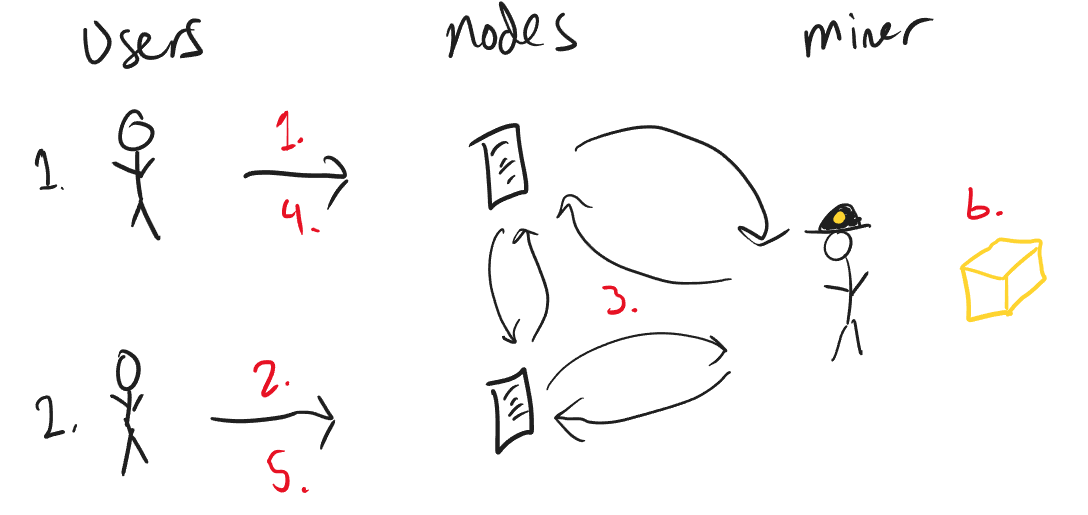
\includegraphics[width=\textwidth]{3_FIGURES/Theory/PGA.PNG}
    \caption{Illustration of Priority Gas Auction}
    \label{PGA}
\end{figure}

\begin{enumerate}
    \item User 1 submits a transaction that executes an arbitrage
    \item User 2 submits a transaction that does the same arbitrage but with a higher gas price
    \item Both transactions get propagated through the network
    \item When user 1 sees user 2 transaction with higher gas price, user 1 submits a new transaction with the same nonce but new gas price.
    \item When user 2 sees user 1 transaction with higher gas price, user 2 submits a new transaction with the same nonce but new gas price.
    \item This behaviour continues until the value of the arbitrage is no longer higher than the cost in gas, or when a miner submits a block that includes a transaction that executes the arbitrage such that the opportunity no longer exists.
\end{enumerate}



% These smart contracts can have any functionality, but the most common applications are financial products. 

% \subsection{Ethereum Request for Comments}

% \subsection{Decentralised Exchanges}


\section{MEV Today}

The Flash Boys 2.0 paper also introduced the concept of Miner Extractable Value (MEV). MEV has since evolved to mean Maximal Extractable Value, since the actor with the power to sequence transactions on the Ethereum network will soon change from miners to validators. MEV refers to the total amount of value block producers can extract from manipulation of transactions. In the paper they describe different methods of extracting that value as well as setting a lower bound for how much value there is to extract. With this lower bound, they argue that the value is great enough to subsidise attacks on the Ethereum network. 

\subsection{Types of MEV}
There are many different types of MEV that all arise from transaction ordering. Some of the most prominent are the following:
\begin{itemize}
    \item \textbf{DEX Arbitrage} As discussed earlier, prices of tokens on different DEX's may be different, thus presenting an opportunity to buy a token cheap on one exchange and sell it for more on another
    \item \textbf{Liquidations} Different smart contracts on Ethereum offer the service of lending capital against collateral. These loans are typically over-collateralised. If the collateral of the loan depreciates in value, any user of the network can submit a transaction to the lending contract in order to liquidate it, effectively repaying the loan. This is done to keep the lending contract solvent. Examples of this are Maker \cite{makerdao} and Aave \cite{Aave}.
    \item \textbf{Sandwich Trading} When a user makes a trade against a DEX, the price of the tokens they traded changes. If you see another users transaction intending to sell token A for token B, you yourself can "sandwich" this transaction by first selling token A for token B, then let the other users transaction sell token A for token B, driving the price of A denominated in B even lower. Then you can buy back token A for less token B than what you got from selling token A initially. This behaviour is frowned upon, since it effectively steals value from the other user, but is none the less profitable.
    \item \textbf{Long tail MEV} Long tail MEV refers to all kinds of exotic ways to extract value. Its called the long tail because most of detectable MEV is made in the categories listed above, but there are many weird MEV strategies that still are profitable. These are typically harder to detect and categorize. 
\end{itemize}

\subsection{MEV-Geth}

As awareness of MEV increased, the PGA's got more and more competitive and the Ethereum network suffered for it. The P2P network propagating transactions got congested by resubmitted transactions with higher gas prices, and block space filled up with reverting transactions that had lost the PGA. In order to mitigate these negative externalities of the PGA's, a research and development organisation called Flashbots made a fork of Geth (an Etherum client written in Go) called MEV-Geth \cite{frontrunMEV}. MEV-Geth allowed for a sealed bid block space auction. It achieved this by introducing new roles in the block building chain:

\begin{itemize}
    \item \textbf{Searchers} Searchers would look in the public mempool for transactions that contained MEV opportunities.
    \item \textbf{Transaction Bundles} When a searcher finds an MEV opportunity they include that transaction in a transaction bundle, along with new transactions extracting the MEV. This bundle is submitted to a bundle pool, a separate mempool for bundles. The bundles include a price that the searcher is willing to pay in order to have the bundle included in certain blocks.
    \item \textbf{Block Templates} Miners running MEV-Geth can now include bundles in their blocks. They choose the bundle which pays them the most, and does not include different bundles containing the same transaction, eliminating reverting transactions due to failed MEV extraction. The rest of the block gets filled with transactions from the public mempool as usual.
\end{itemize}

Not all new blocks on Ethereum today have bundles in them, but a significant amount do. With MEV-Geth in the loop, the transaction lifecycle looks something like this \cite{auctionoverview}:


\begin{figure}[H]
    \centering
    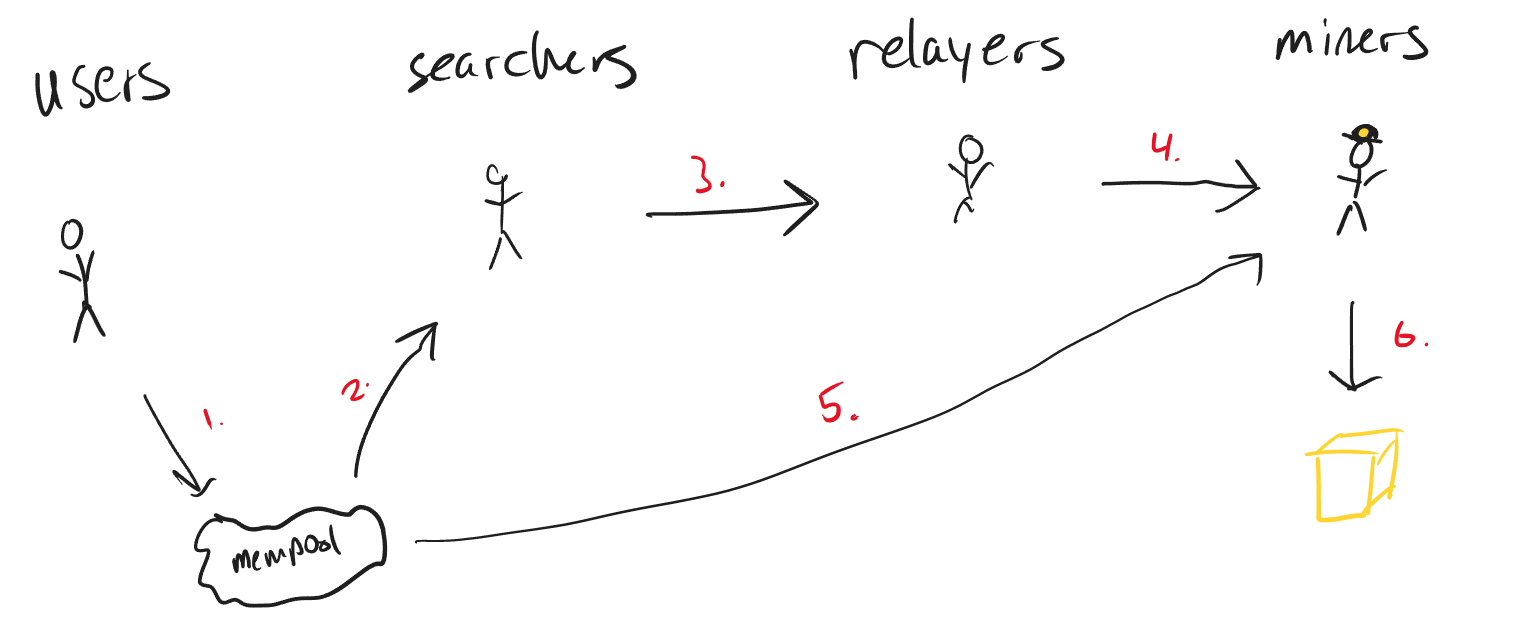
\includegraphics[width=\textwidth]{3_FIGURES/Theory/mevgeth.PNG}
    \caption{Transactions in a MEV-Geth setting}
    \label{mevgeth}
\end{figure}

\begin{enumerate}
    \item A users submits a transaction to the mempool
    \item A searcher finds an MEV opportunity in the mempool and creates a bundle with the transaction(s)
    \item It sends the bundle to a relayer
    \item The relayer propagates the bundle to miners
    \item The miner takes the bundle and transactions from the mempool and includes them in the block template
    \item The miner makes a block based on the block template and gets the fee from the MEV bundle and the gas fees from the included mempool transactions
\end{enumerate}

\subsection{MEV-Inspect}

Along with MEV-Geth, Flashbots build another piece of open sourced software called MEV-Inspect. The goal of this was to "Illuminate the Dark Forest". In other words, to make data quantifying the extent of MEV extraction on Ethereum available to everyone. It worked by having a crawler look through transactions in order to categorise them and put them in a database for further analysis. This was a best effort attempt to set a lower bound for actualised MEV. More precise estimations of actualised MEV is hard, because the long tail MEV is so hard to classify. 


\section{Cross Domain MEV}
In late 2021, a group of researchers published a paper entitled "Unity is Strength: A Formalization of Cross-Domain Maximal Extractable Value" \cite{crossdomainMEV}.  Based on this paper and multiple talks from the recent conference \cite{mevday} which we attended in Amsterdam, we will in this section, shed some light on the concepts behind Cross Domain MEV.

\subsection{Domains}
Traditionally when people have talked about MEV, it was in a single domain. MEV searchers have been running their MEV bots on many different chains, playing games to out-compete each other on latency or gas price. But as the development of Ethereum is moving along the road map, a picture of the modular Ethereum future becomes clearer. Ethereum today already supports a wide range of different execution environments and many different Layer 2 solutions. These solutions submit data to Ethereum so that their state can be verified, but are in essence their own chains. For now most of these domains have centralised aspects to them eg. Arbitrums sequencer, which is run by the Arbitrum team. This means there are actors with sequencing rights present today. As we saw in the previous section, having the sequencing rights is valuable. Whoever orders the transactions can extract the MEV. 

\subsection{Leg risk}
When you perform an arbitrage on Ethereum today, you compete with other searchers on how efficiently you can do it, and on how much of the profit you are willing to pay to the miner. You do this buy submitting bundles. These bundles are executed atomically, meaning all the transactions in the bundle are executed without failing, or all the transactions in the bundle gets reverted. This means that you are never stuck half way through an arbitrage with a token that you do not really want to own. When you introduce multiple domains to your arbitrage opportunities you reintroduce this risk. Lets take an example:

\begin{figure}[H]
    \centering
    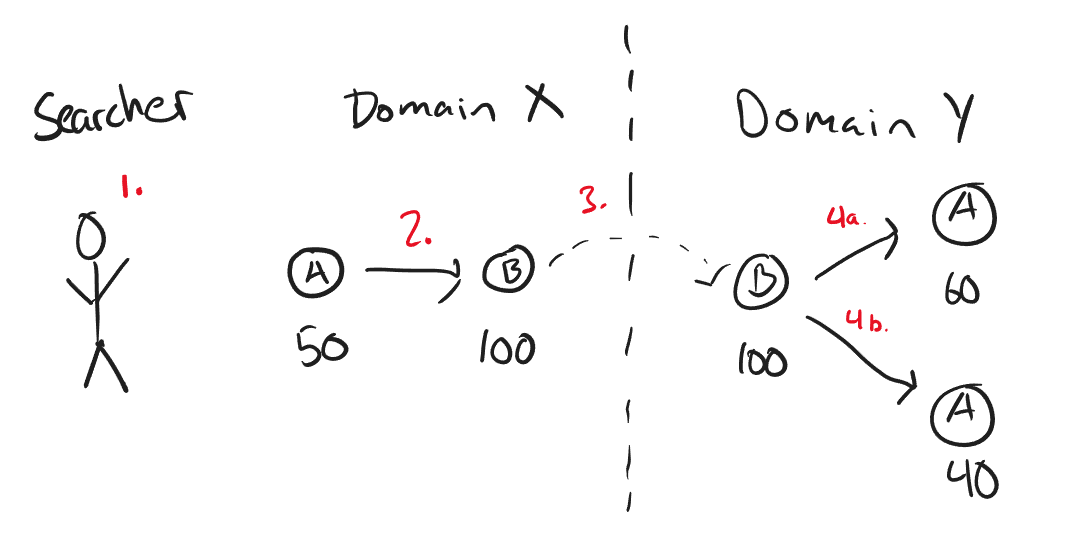
\includegraphics[width=\textwidth]{3_FIGURES/Theory/legrisk.PNG}
    \caption{Illustration of leg risk}
    \label{legrisk}
\end{figure}

\begin{enumerate}
    \item You, as a searcher, see that the price of token A is cheaper denominated in token B in domain Y compared to domain X. You wish to take advantage of this to make profit
    \item You swap 50 A tokens for 100 B tokens in domain X
    \item You transfer the newly acquired B tokens to domain Y
    \item Now one of two scenarios await you
    \begin{enumerate}[label=\alph*]
        \item The price of token A denominated in B has not changed since your journey started, and you get the profit you expected
        \item The state of domain Y has changed since you started your journey and you take a loss on the last leg of the arbitrage.
    \end{enumerate}
\end{enumerate}

Leg risk is present when you go between domains, with a notable exception: If you control the sequencing of one domain, you can refrain from updating the state of that domain. This means that Arbitrum could in theory look for the price of a token to be favourable on another domain compared to Arbitrum, wait for a transaction taking advantage of this to go through on the second domain, and then finish the last leg of the arbitrage without assuming any leg risk. If we control the sequencing of one domain, we can effectively perform atomic cross domain arbitrages, where users that do not control sequencing assume leg risk by doing so. 

\subsection{Implications}

If you consider a Centralised Exchange (CEX) to be a domain, its clear that its possible for such actors to arbitrage between themselves and DEX'es in other domains without assuming leg risk. One fear is that when Ethereum moves from PoW to PoS, the allure of capital efficient Liquid Staking Derivatives (LSDs) will aggregate more and more validating power to centralised entities. Many people today stake through CEX's to reduce complexity and assume less risk. This means that these CEX's in the future will have more power over the sequencing than what normal users of the network will have. 